\newpage
\subsection*{Вывод}
В качестве вывода можно выделить некоторые особенности написания скриптов на bush: так например, вокруг знаков присвоения недопустимо ставить пробелы, а при написании условия в if напротив перед скобками следует ставить пробелы, также были изучены способности заносить в циклы и условия не только математические операции, но и выполнение/невыполнение различных команд. Конечно были изучены структура и синтаксис циклов, условий, функций и некоторых операций для написания скриптов, о чем изложено в работе выше. \\

Вкупе с приведенными ранее моментами можно сказать о том, что нами были изучены и освоены основы написания скриптов в оболочке bush. А также были решены небольшие практические задачи, подробнее о которых можно узнать из пунктов 1-3. \\

 \begin{center}
		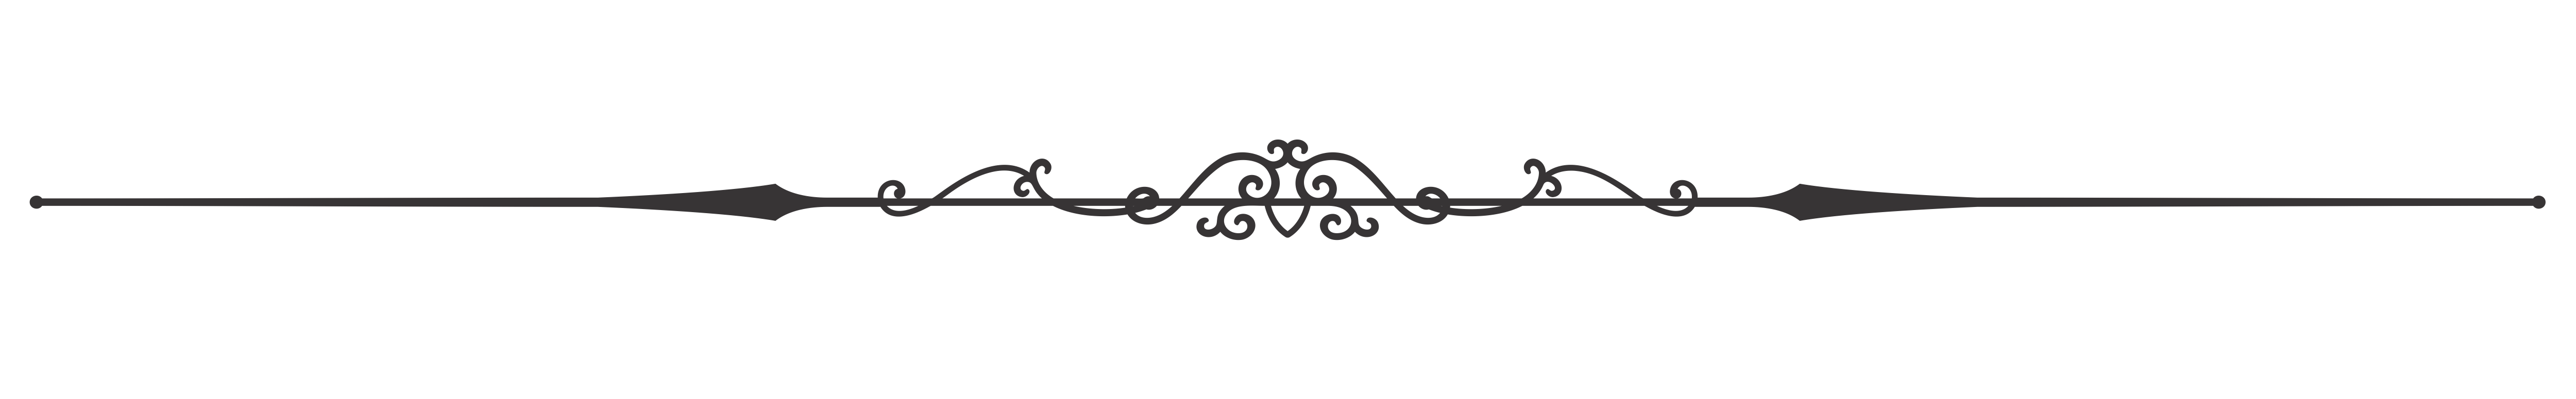
\includegraphics[width=0.8\textwidth]{line.png}
	\end{center}

 \vspace{1.5cm}
 \centerline{Спасибо за внимание}